At this point the robot was able to explore and discover its environment by itself, but there were some details that we could improve.

\section{Inaccessible frontiers}

Sometimes a frontier is found in an inaccessible place, then the robot will go the closest to the frontier it can and the closest frontier will always remain an inaccessible one, the robot will then stay stuck.

To fix this issue we had to find a way to detect when the robot stays stuck and then delete the frontier that it is trying to reach.

We created a new process called 'frontiers limiter' that would be executed in the back ground, it runs every second and memorise the actual position of the robot.
It communicates with the goal planner which send to it the last closest frontier as soon as it is computed, the frontiers limiter sends to the goal planner a list of all the cells to ignore when it is building the frontiers.
It only memorise the last 14 positions of the robot, which make it delete every position older than 14 seconds.
Once it has memorised 14 positions it computes $\Delta x$ and $\Delta y$ and if those $\Delta$s are bellow 5 meters for both of them the robot is considered as stuck, because it means that the robot stayed in a square of 5 meters by 5 meters for the last 14 seconds.
Once the robot is detected as stuck the frontier limiter will find tell the goal planner to find the biggest frontier and nor the closest.
That can either fix the situation or the robot will still be stuck.
If the robot is detected as being stuck twice in a row this time the closest frontier will be deleted in this way: we go through all the points in the frontier and add all the cells in a radius of 6 cells around each point to the list of cells to ignore, then it sends the updated list to the goal planner.
In that way the goal planner will ignore the cells in the list when it is building the frontiers in the future.

\section{Disadvantages of using potential fields}

We knew that using potential fields could be a problem because of the local minimums in which the robot could stay stuck.
Despite that we decided that we wanted to try to implement it to try and see by ourselves what kind of problems we could encounter and the solutions that we could find.

We found a solution which works most of the time for the inaccessible frontiers but there still is an issue that we could not solve.
It is when the robot goes in the garage area, here the robot usually wants to go to a frontier that is outside of the garage and it stays stuck inside.
It is a problem that we would not have had if we chose to implement a path planning and a path tracking process.

There is also the case in which the goal is right behind an obstacle, in that case the robot can stay stuck.

\section{Results obtained}

This is an image of the map of the area explored by the robot, in this run the robot managed to enter, explore and go out from the garage without much troubles.

\FloatBarrier
\begin{figure}
    \centering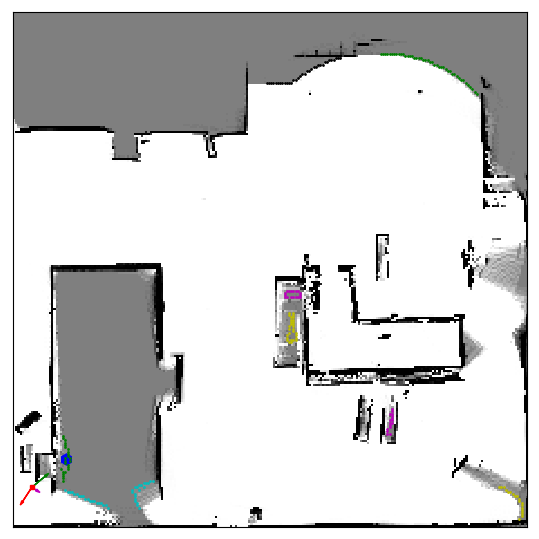
\includegraphics[width=\textwidth]{robot_explored_map.png}
    \label{fig:robot_explored_map}
    \caption{Robot explored map}
\end{figure}
\FloatBarrier

